\section{Ejercicio 3}

\subsection{Problema}

\subsection{Algoritmo e intuición}

\subsubsection*{Pseudocódigo}

Sea la clase $Grafo = <Vertices, Aristas, ListaAdyacencia>$
	donde Vertices y Aristas son Enteros que representan la cantidad de vertices y aristas del grafo y
	ListaAdyacencia es un $Vector<Lista<Par<Entero, Entero>>>$ donde
	el tamano del vector es Vertices y por cada arista que conecta nodos v 
	y w del grafo representado, ListaAdyacencia[v] incluye $<e, w>$ y
	ListaAdyacencia[w] incluye $<e, v>$ donde $e$ es el número de arista (entre 0 y Aristas-1).

\begin{algorithm}[]
    \caption{ResolverQueries}
    \Input{Grafo $grafo$, Queries $queries$}
    $Vector<Bool>$ $puentes \gets [false,...,false]$ con size grafo.Aristas \;
	$Vector<Entero>$ $depth \gets [-1,...,-1]$ con size grafo.Vertices \;
	$Vector<Entero>$ $low \gets [-1,...,-1]$ con size grafo.Vertices \;
	\emph{CalcularPuentesDFS$(grafo, puentes, depth, low, 0, 0, 0)$} \;
	$Vector<Entero>$ $componente\_puente\_del\_vertice \gets [-1,...,-1]$ de size grafo.Vertices \;
	$Vector<Entero>$ $vertices\_del\_componente\_puente \gets [0,...,0]$ de size grafo.Vertices \;
	$Variable$ $Global$ $Entero$ $contador\_componentes \gets 0$ \;
	\emph{CalcularComponentesPuenteDFS$(grafo, puentes, componente\_puente\_del\_vertice, $ $ vertices\_del\_componente\_puente, 0, contador\_componentes, 0)$} \;
	\For{$query$ en $queries$} {
		\If{$query.tipo$ == A} {
			$Vector<Bool>$ $visitado \gets [false,...,false]$ con size grafo.Vertices \;
			\emph{Imprimir PuentesEntreNodos$(grafo, puentes, visitado, query.esquina1, query.esquina2, query.esquina1)$}
		}
		\If{$query.tipo$ == B} {
			\emph{Imprimir $puentes[query.calle]$}
		}
		\If{$query.tipo$ == C} {
			$Entero$ $n$ \;
			$n \gets vertices\_del\_componente\_puente[componente\_puente\_del\_vertice[query.esquina]]$ \;
			\emph{Imprimir n-1}
		}
	}
\end{algorithm}

\begin{algorithm}[]
    \caption{CalcularPuentesDFS}
    \Input{Grafo $grafo$, Vector$<Bool>$ $puentes$, Vector$<Entero>$ $depth$, Vector$<Entero>$ $low$, Entero $v$, Entero $d$, Entero $padre$}
    $depth[v] \gets d$ \;
	$low[v] \gets d$ \;
	\For {$<e, w>$ en $grafo.ListaAdyacencia[v]$ tal que $w$ != $padre$} {
		\eIf{$depth[w]$ == -1}{
			\emph{CalcularPuentesDFS$(grafo, puentes, depth, low, w, d+1, v)$} \;
			$low[v] \gets min(low[v], low[w])$ \;
			\If {$low[w] >= depth[w]$} {
				$puentes[e] \gets true$
			}
		}{
			$low[v] \gets min(low[v], depth[w])$ \;
		}
	}
\end{algorithm}

\begin{algorithm}[]
    \caption{CalcularComponentesPuenteDFS}
    \Input{Grafo $grafo$, Vector$<Bool>$ $puentes$, Vector$<Entero> componente\_puente\_del\_vertice$, Vector$<Entero> vertices\_del\_componente\_puente$, Entero $v$, Variable Global Entero $contador\_componentes$, Entero $componente\_actual$}
    $componente\_puente\_del\_vertice[v] \gets componente\_actual$ \;
    $vertices\_del\_componente\_puente[componente\_actual]++$ \;
    \For {$<e, w>$ en $grafo.ListaAdyacencia[v]$} {
    	\If {$componente\_puente\_del\_vertice[w]$ == -1} {
			\eIf {$puentes[e]$} {
				$contador\_componentes++$ \;
				$Entero$ $componente \gets contador\_componentes$ \;
				\emph{CalcularComponentesPuenteDFS($grafo, puentes, componente\_puente\_del\_vertice,$ 
				$vertices\_del\_componente\_puente, w, contador\_componentes, componente$)} \;
			}{
				\emph{CalcularComponentesPuenteDFS($grafo, puentes, componente\_puente\_del\_vertice,$ 
				$vertices\_del\_componente\_puente, w, contador\_componentes, componente\_actual$)}
			}
		}
    }
\end{algorithm}

\begin{algorithm}[H]
    \caption{PuentesEntreNodos}
    \Input{Grafo $grafo$, Vector$<Bool>$ $puentes$, Vector$<Bool>$ $visitado$, Entero $src$, Entero $dst$, Entero $actual$}
    $visitado[actual] \gets true$ \;
    \If {$actual == dst$} {
    	\Return{0}
    }
    $Entero$ $ans \gets -1$ \;
    \For {$<e, w>$ en $grafo.ListaAdyacencia[v]$} {
    	\If {$visitado[w]$ == $false$} {
			$Entero$ $rec \gets$ PuentesEntreNodos$(grafo, puentes, visitado, src, dst, w)$ \;
			\If{$rec$ != -1} {
				$ans \gets puentes[e]$ ? $rec+1$ : $rec$
			}
		}
    }
    \Return{ans}
\end{algorithm}

\subsubsection*{Estrategia}

\subsection{Correctitud}

\subsubsection*{ResolverQueries}
Esta es la función principal del algoritmo. Dado el grafo y las queries de entrada se crea un vector $puentes$ 
que contiene para cada arista si es puente o no, lo cual se quiere calcular a continuaci\'on. \\
Es importante notar que por la forma en que se crea la clase Grafo y se rellena, cada eje tiene un número 
único entre 0 y la cantidad de aristas menos uno. \\
Luego se crean dos vectores $depth$ y $low$ de tamaño cantidad de vértices del grafo. Con esto se calculan los
ejes puente mediante la funci\'on CalcularPuentesDFS. El nodo inicial de CalcularPuentesDFS es arbitrario 
mientras sea el mismo que el padre inicial, por lo cual se define al nodo 0 como el inicial. Además queremos 
que el $depth$ inicial sea 0 ya que es la profundidad inicial de los nodos según el algoritmo para calcular 
Componentes Biconexas Maximales explicado en clase, que es en definitiva el esquema que sigue la funcio\'n 
CalcularPuentesDFS. \\
Habiendo calculado los aristas puente, ahora se quiere calcular para cada nodo e1, la cantidad de nodos e2 
tales que de cortar una sola arista, sea cual sea, seguir\'a habiendo un camino de e1 a e2. \\
Como el grafo es conexo, las nodos inicialmente están conectados. Dada el nodo e1, si existe una arista tal que al 
cortarla e1 y otro nodo se desconectan entonces seguro que esa arista es un puente (por la definición de puente). 
De hecho, si corto una arista que no es puente, el grafo sigue siendo conexo. \\
El problema es cuando e1 y e2 forman un puente o pertenecen a diferentes componentes biconexas maximales, es decir, 
cuando hay un puente entre ellos. Más aún, e1 y e2 siguen estando conectados no importa cual arista sea cortada
si y solo si pertenecen a una misma componente biconexa maximal que no sea un puente. \\
Por esto se puede concluir que es posible seguir llegando de un nodo e1 a otro e2 habiendo cortado una calle 
cualquiera, mientras no hayan aristas puente entre ellos. Si hay un arista puente entre ellos, cortarlo basta para desconectarlos. \\
Con esta motivación definimos los Bridge Components del grafo. Estos componentes se obtienen condensando cada componente biconexa 
maximal que no es un puente en un solo nodo. \\

Ejemplo:\\
\begin{figure}[H]
\centering
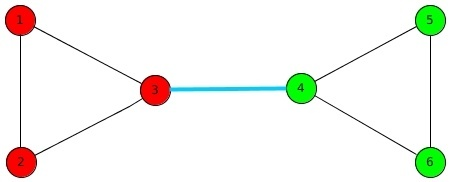
\includegraphics[width=90mm]{./img/bridge_comp_1.jpeg}
\caption{Grafo original}
\end{figure}
\begin{figure}[H]
\centering
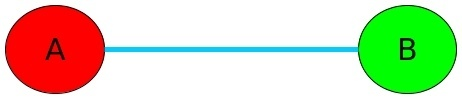
\includegraphics[width=90mm]{./img/bridge_comp_2.jpeg}
\caption{Grafo condensado en Bridge Components}
\end{figure}

El algoritmo CalcularComponentesPuenteDFS hace esto guardando para cada nodo 
a qué Bridge Component pertenece en el vector $componente\_puente\_del\_vertice$ y para cada uno de esos componentes, 
$vertices\_del\_componente\_puente$ guarda cuántos nodos tiene ese componente. \\
Ahora bien, los nodos dentro de cada Bridge Component están conectados de manera tal que no hay puentes entre ellos,
por lo cual si corto cualquier arista del grafo siguen estando conectados entre si.

Finalmente, el algoritmo resuelve las queries según su tipo correspondiente:
\begin{itemize}
	\item[A: ] dado que se quiere imprimir la cantidad de calles que, en caso de ser cortadas impiden llegar de la 
	esquina e1 a e2, cuenta mediante la función PuentesEntreNodos y el vector $puentes$, los puentes entre los nodos 
	del grafo que representan esas esquinas.
	\item[B: ] se fija en el vector $puentes$ si la calle es un puente o no y lo imprime.
	\item[C: ] dada una esquina e1 se quiere imprimir la cantidad de esquinas e2 tales que de cortar una calle cualquiera 
	sigue habiendo camino de e1 a e2. Como explicamos esto es exactamente la cantidad de nodos en el Bridge Component del
	grafo, que son justamente los nodos e2 que están conectados a e1 sin puentes entre e1 y e2, entonces sin importar
	qué calle se corte, seguirán estando conectados. Los demás nodos son posibles de desconectar de e1 cortando alguno
	de los aristas puentes entre e1 y esos nodos. Notar que a esta cantidad se le resta 1 para no contar a e1 en su 
	propio Bridge Component.
\end{itemize}

\subsubsection*{CalcularPuentesDFS}

\subsubsection*{CalcularComponentesPuenteDFS}

\subsubsection*{PuentesEntreNodos}

\subsection{Complejidad}

\subsection{Casos de prueba}
